\documentclass{article}


% \usepackage{arxiv} # uncomment for preprint

\usepackage[utf8]{inputenc} % allow utf-8 input
\usepackage[T1]{fontenc}    % use 8-bit T1 fonts
% \usepackage{hyperref}       % hyperlinks
\usepackage{url}            % simple URL typesetting
\usepackage{booktabs}       % professional-quality tables
\usepackage{amsfonts}       % blackboard math symbols
\usepackage{nicefrac}       % compact symbols for 1/2, etc.
\usepackage{microtype}      % microtypography
\usepackage{lipsum}
\usepackage{graphicx}
\usepackage{subfigure}
\usepackage{amsmath}

\usepackage{placeins}
% \usepackage{algpseudocode}
\usepackage{algorithm}

% \algnewcommand\algorithmicforeach{\textbf{foreach}}
% \algdef{S}[FOR]{ForEach}[1]{\algorithmicforeach\ #1\ \algorithmicdo}


\usepackage{hyperref}


\begin{document}

\renewcommand{\thetable}{S\arabic{table}}

\renewcommand{\thefigure}{S\arabic{figure}}

\section{Results}

\begin{figure}[ht!]
    \centering
    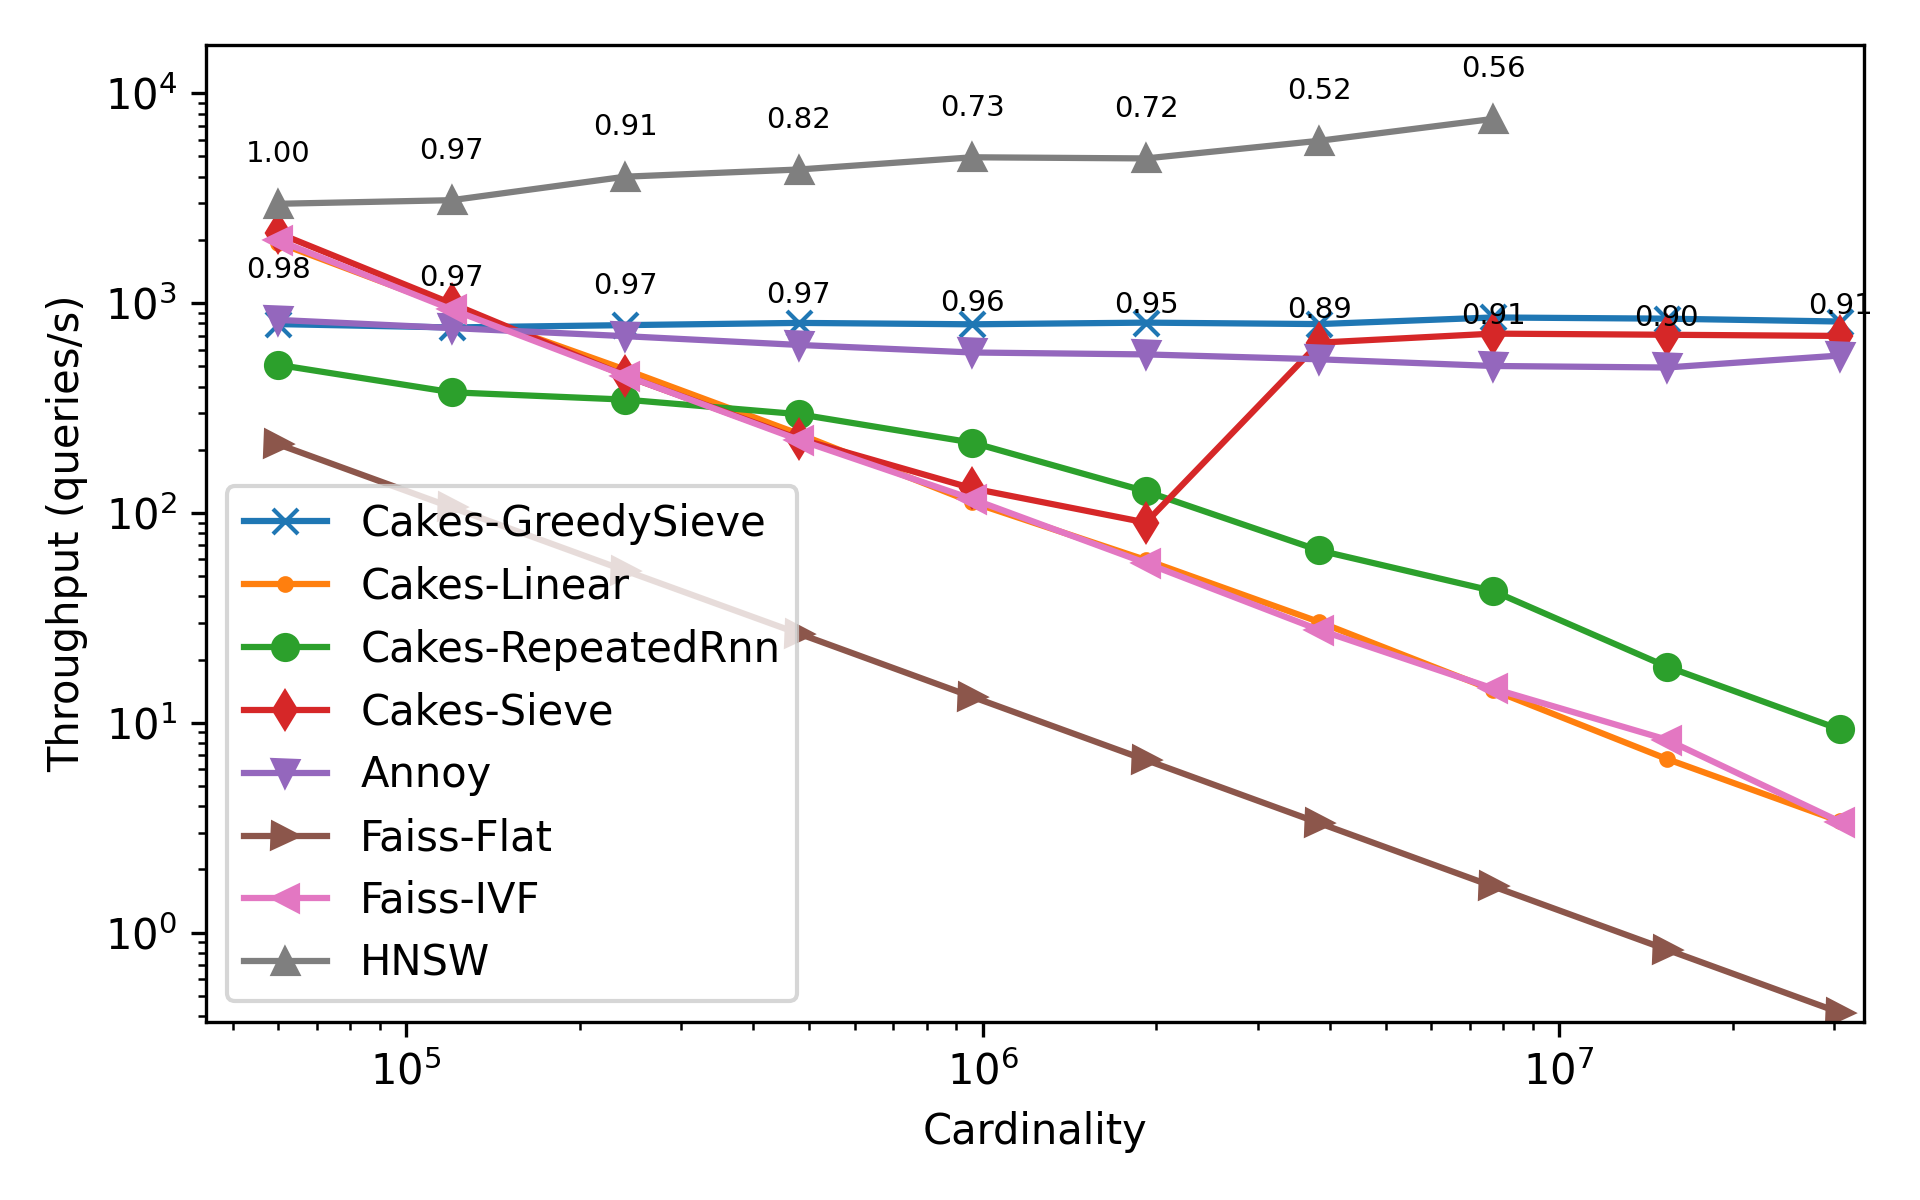
\includegraphics[width=3.4in]{plots/fashion-mnist-knn-100.png}
    \caption{
        Scaling behavior of algorithms on fashion-mnist with $k=100$. 
    }
    \label{fig:supplement:fashion-mnist-k-100}
\end{figure}

\begin{figure}[ht!]
    \centering
    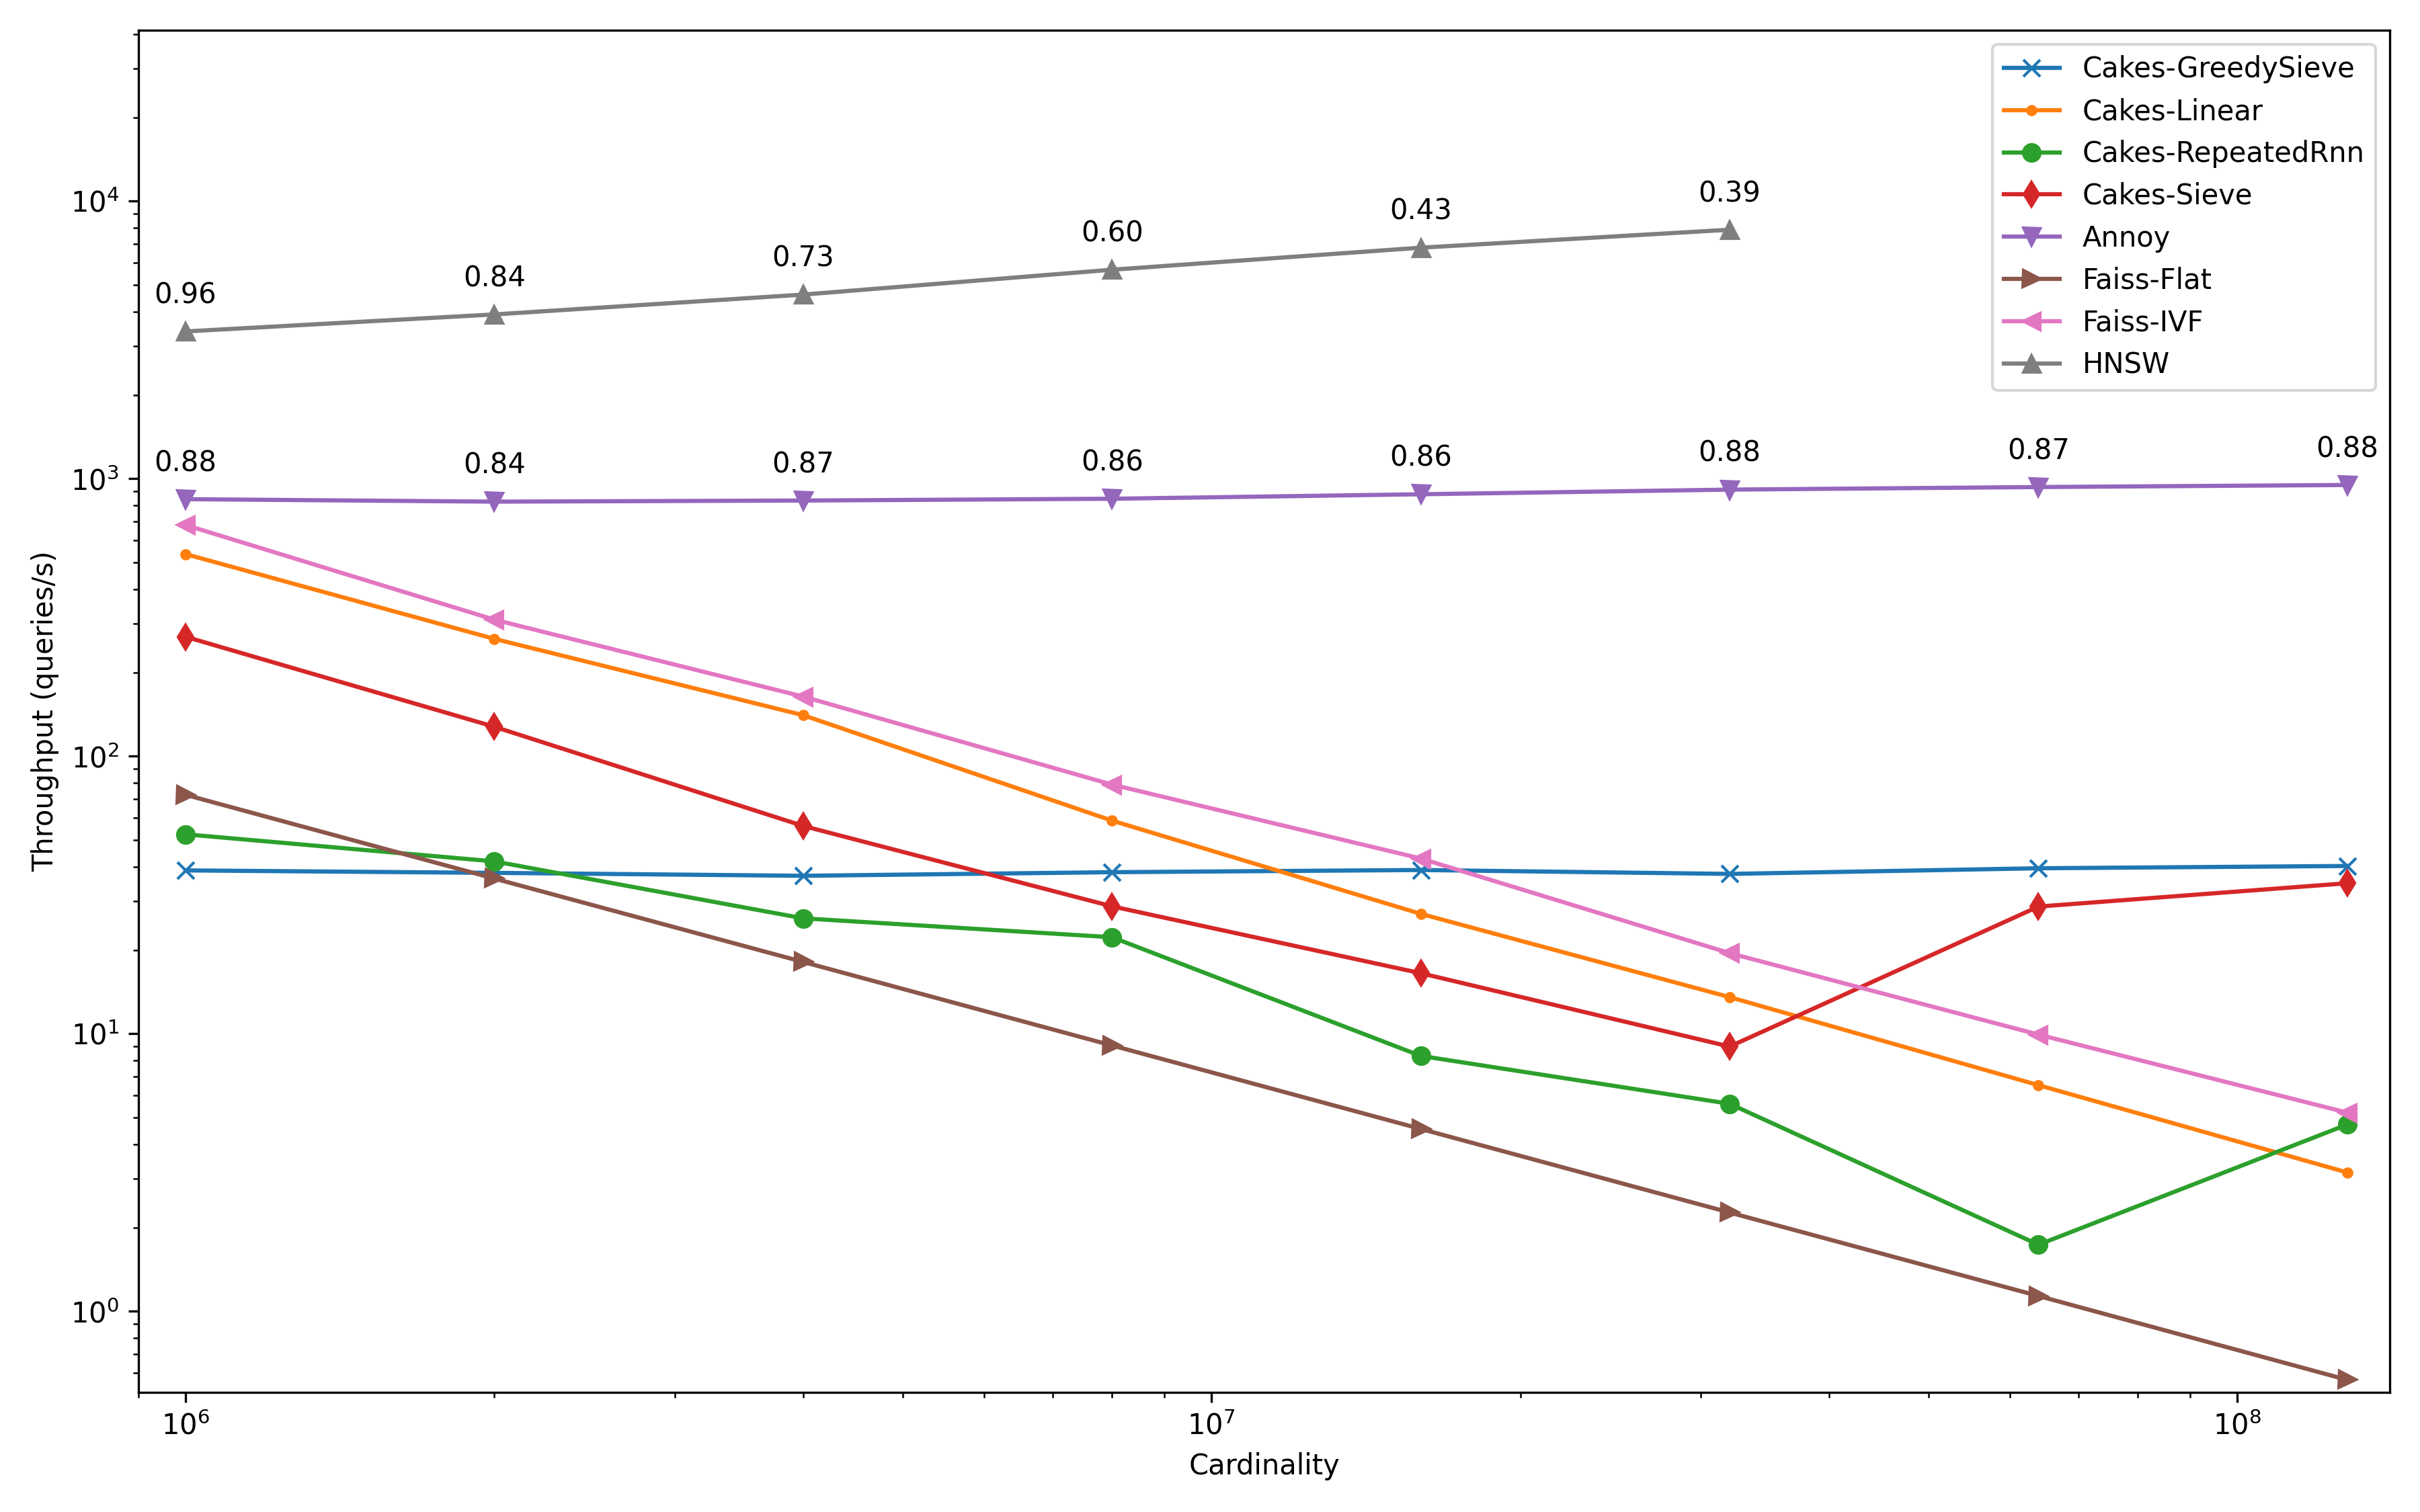
\includegraphics[width=3.4in]{plots/sift-knn-100.png}
    \caption{
        Scaling behavior of algorithms on sift with $k=100$. 
    }
    \label{fig:supplement:sift-k-100}
\end{figure}

\begin{figure}[ht!]
    \centering
    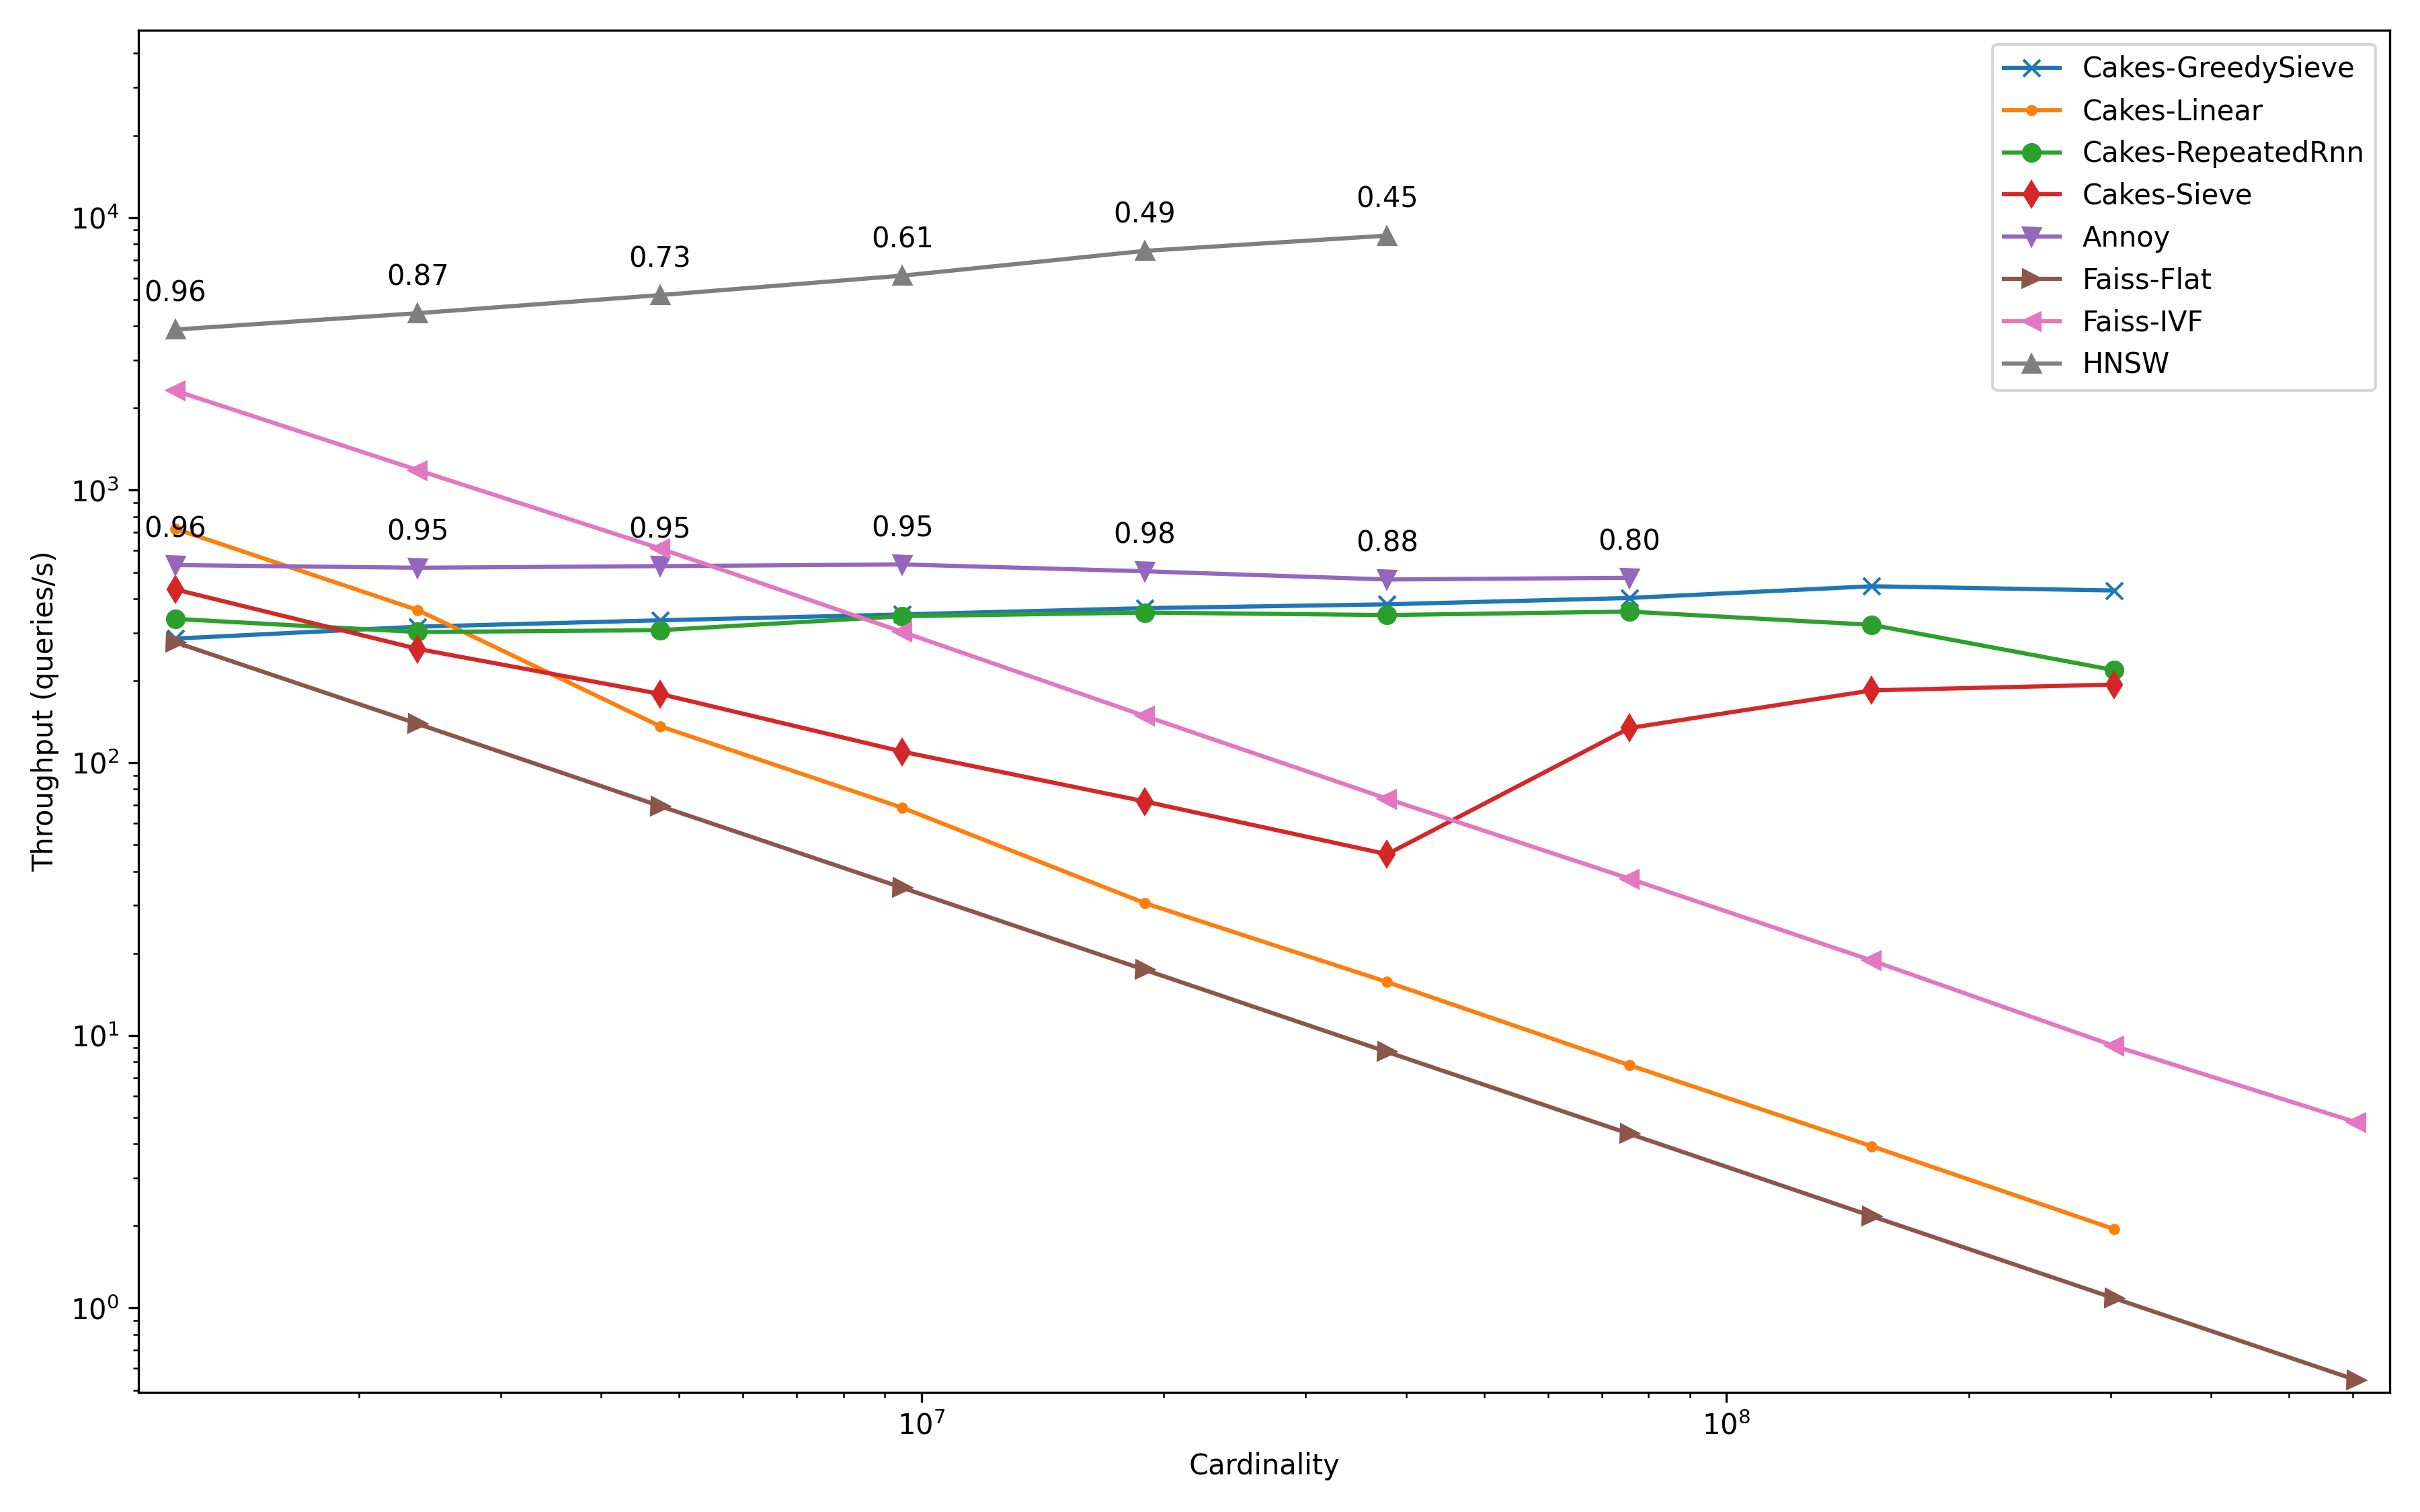
\includegraphics[width=3.4in]{plots/glove-25-knn-100.png}
    \caption{
        Scaling behavior of algorithms on glove-25 with $k=100$. 
    }
    \label{fig:supplement:glove-25-k-100}
\end{figure}

\begin{figure}[ht!]
    \centering
    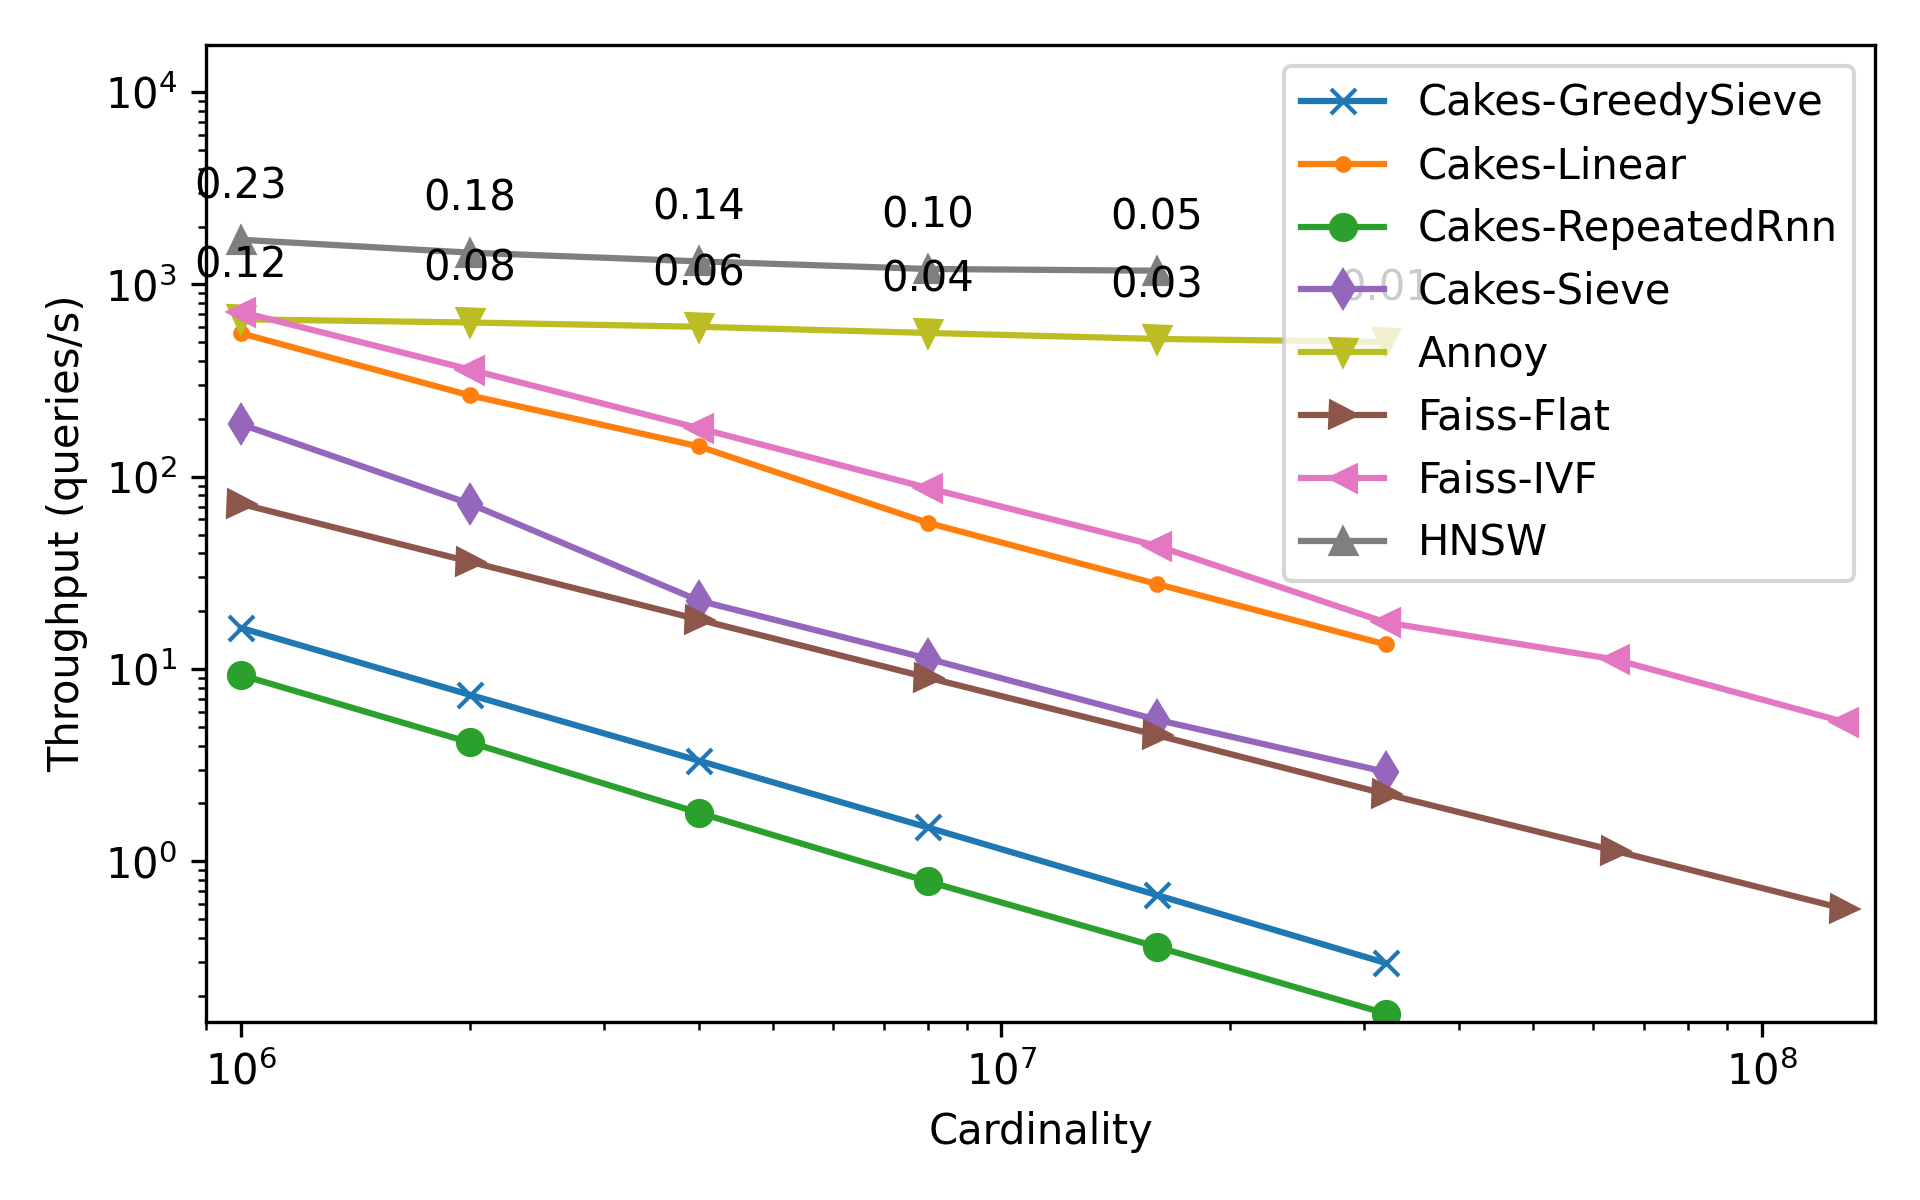
\includegraphics[width=3.4in]{plots/random-knn-100.png}
    \caption{
        Scaling behavior of algorithms on random with $k=100$. 
    }
    \label{fig:supplement:random-k-100}
\end{figure}

\begin{figure}[ht!]
    \centering
    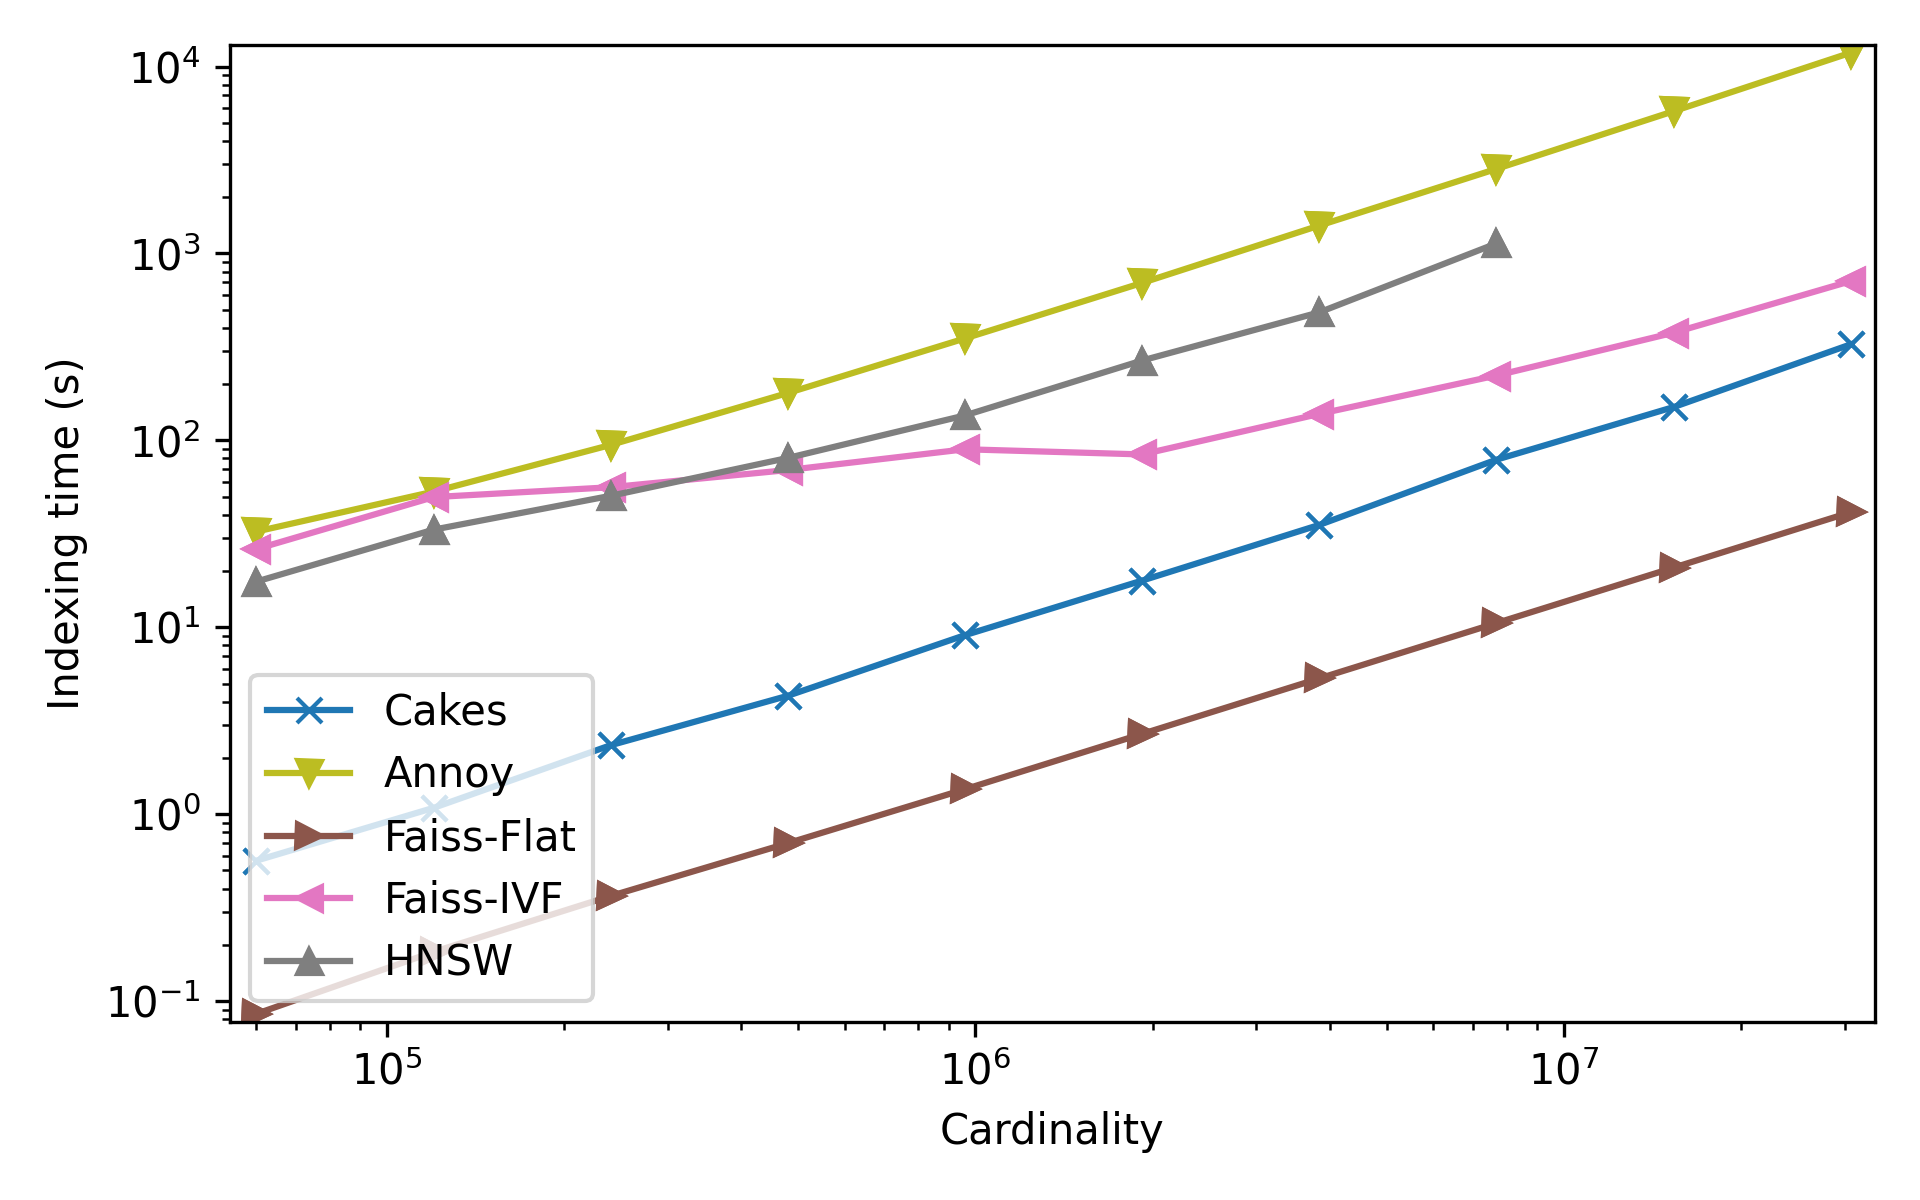
\includegraphics[width=3.4in]{plots/fashion-mnist-indexing.png}
    \caption{
        Indexing time for algorithms on fashion-mnist dataset. 
    }
    \label{fig:supplement:fashion-mnist-indexing}
\end{figure}

\begin{figure}[ht!]
    \centering
    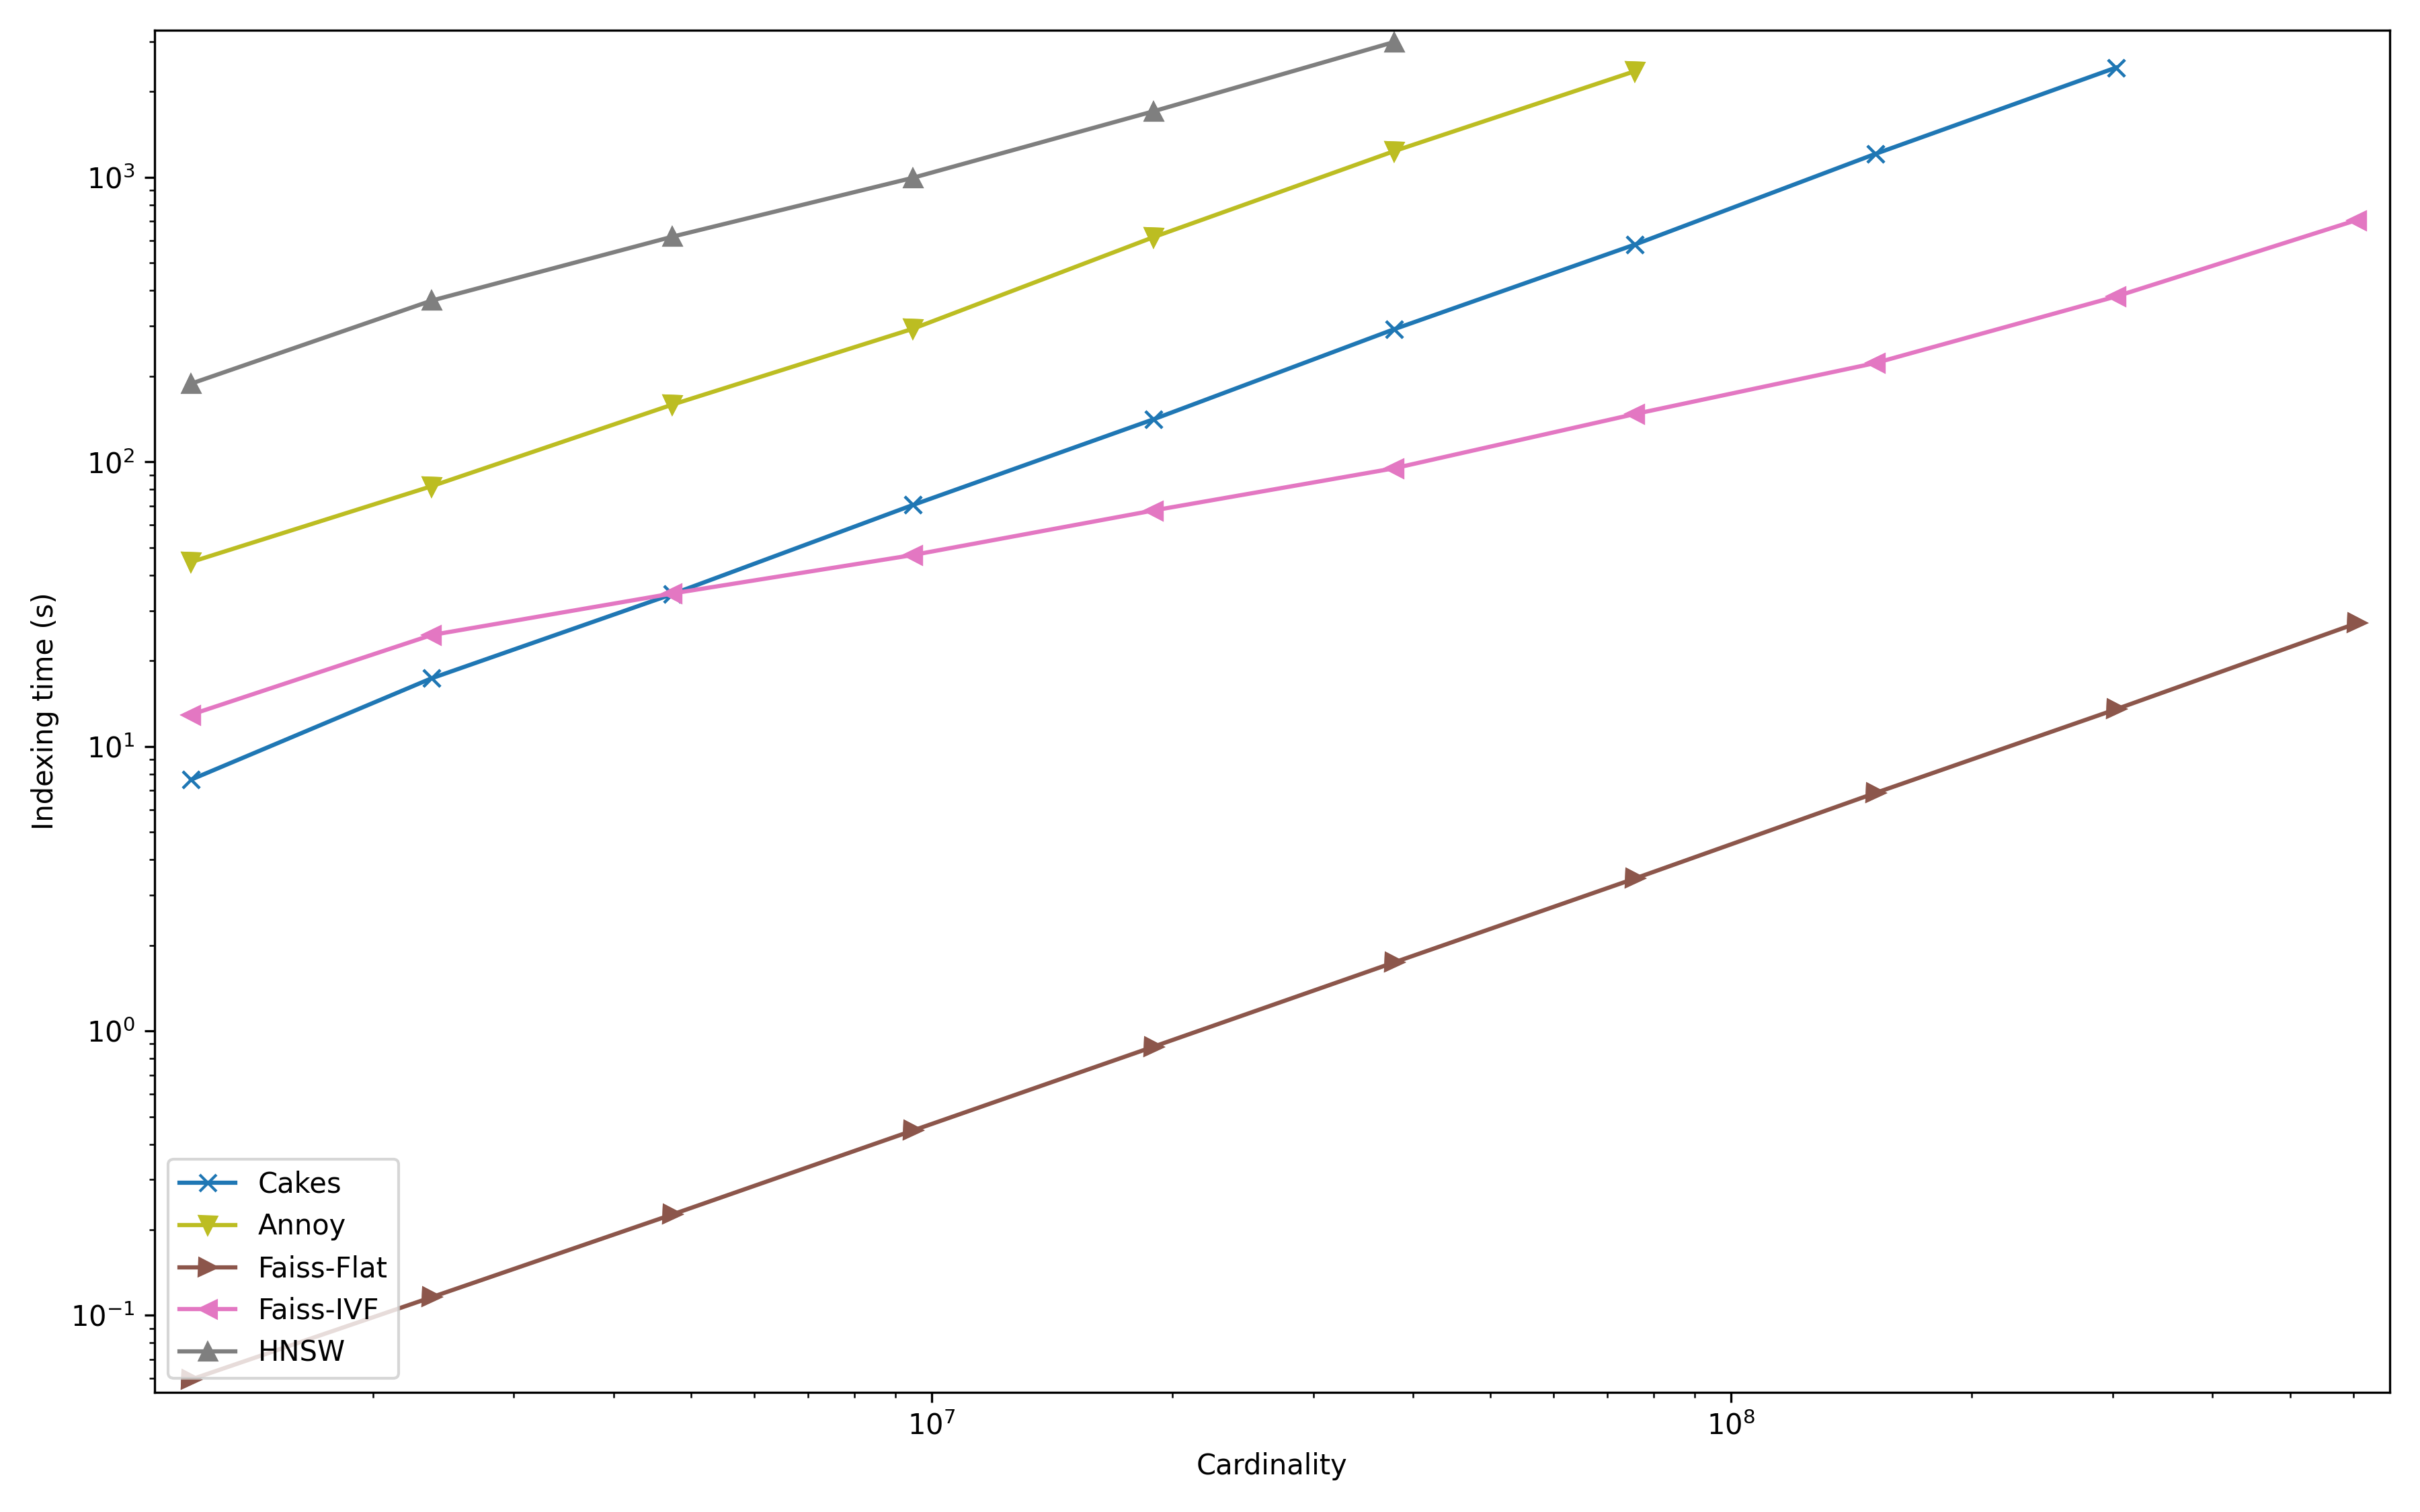
\includegraphics[width=3.4in]{plots/glove-25-indexing.png}
    \caption{
        Indexing time for algorithms on glove-25 dataset. 
    }
    \label{fig:supplement:glove-25-indexing}
\end{figure}


\begin{figure}[ht!]
    \centering
    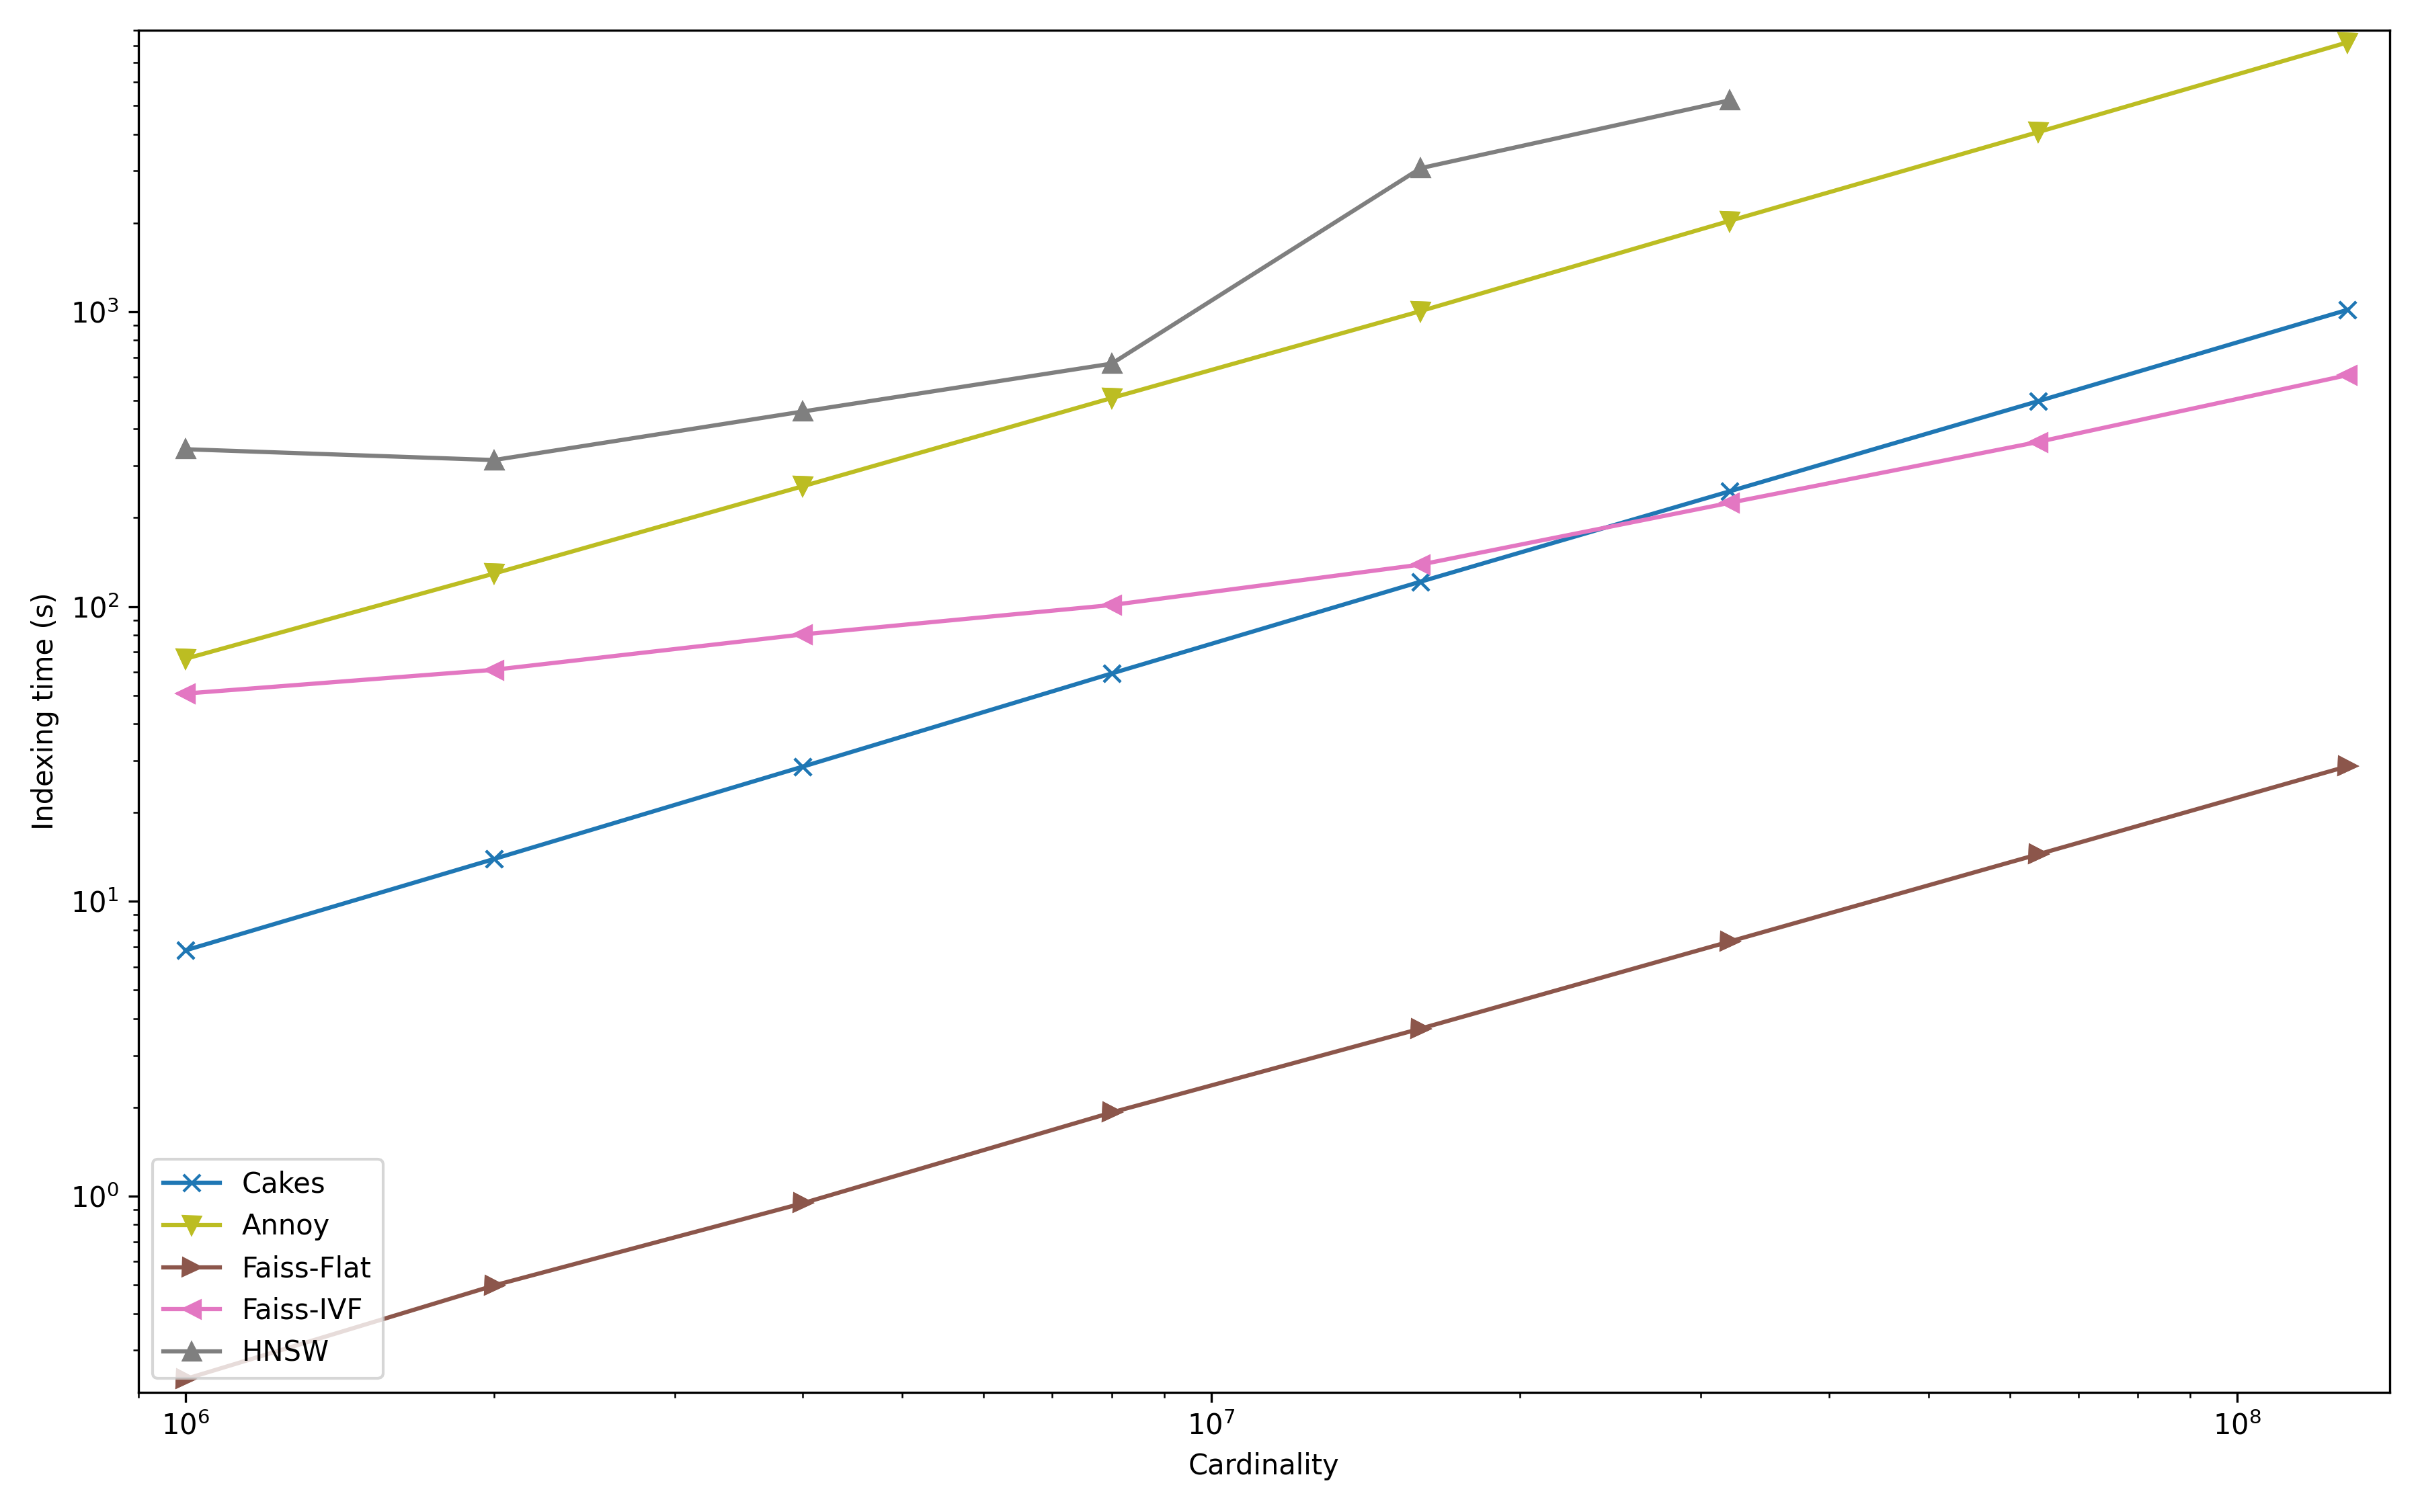
\includegraphics[width=3.4in]{plots/sift-indexing.png}
    \caption{
        Indexing time for algorithms on sift dataset. 
    }
    \label{fig:supplement:sift-indexing}
\end{figure}

\begin{figure}[ht!]
    \centering
    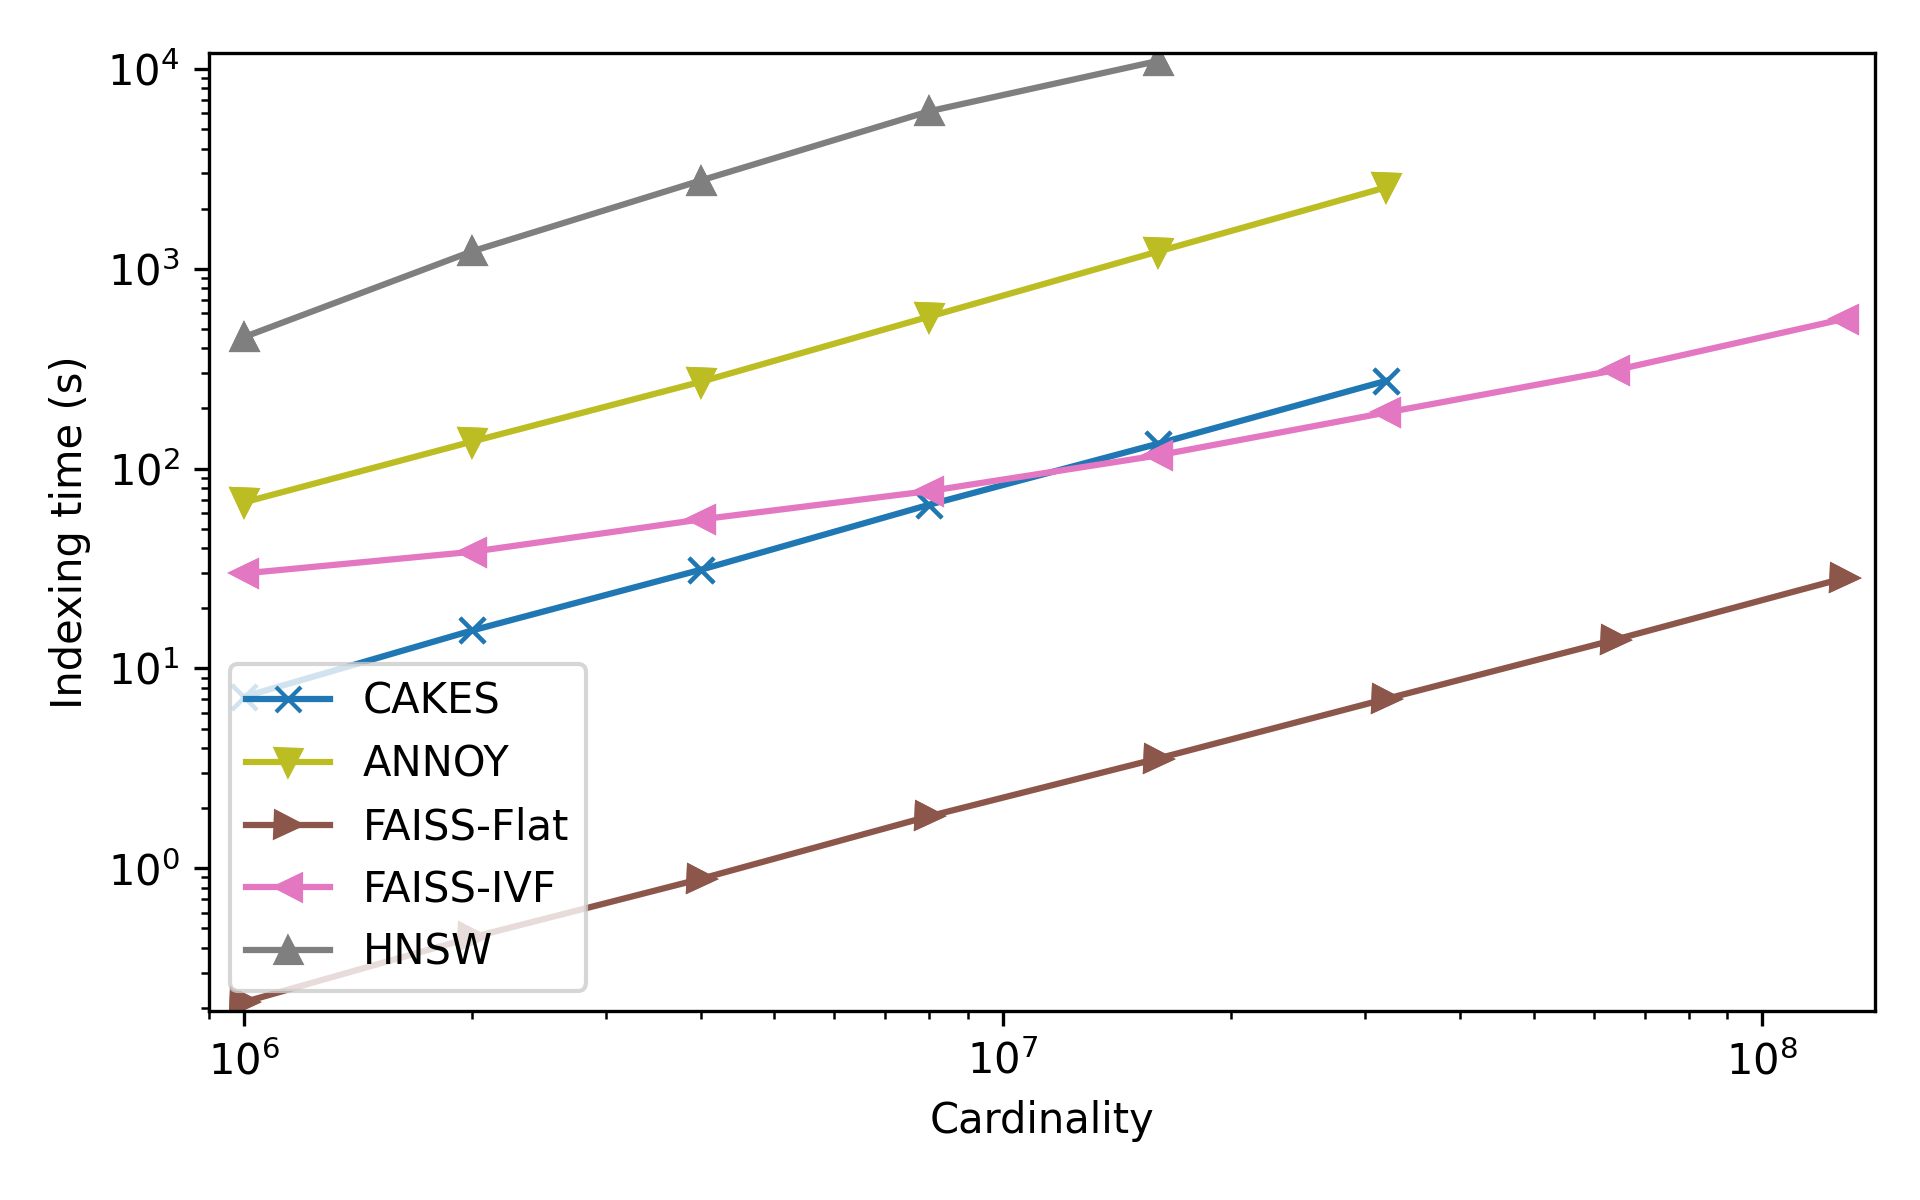
\includegraphics[width=3.4in]{plots/random-indexing.png}
    \caption{
        Indexing time for algorithms on random dataset. 
    }
    \label{fig:supplement:random-indexing}
\end{figure}

\end{document}